\documentclass[12pt,a4paper]{article}
\usepackage[utf8x]{inputenc}
\usepackage[english,hebrew]{babel}
\usepackage{graphicx}
\usepackage{verbatim}
\usepackage{url}
\usepackage{bm}

\graphicspath{{images/}}

\usepackage{tikz}
\usetikzlibrary{external,intersections,patterns}
\tikzexternalize[prefix=tikz/]

% Use stealth arrows
\tikzset {
  >=stealth
}

\textwidth=15.5cm
\textheight=23cm
\topmargin=0pt
\headheight=0pt
\oddsidemargin=2em
\headsep=0pt
\parindent=0pt
\renewcommand{\baselinestretch}{1.1}
\setlength{\parskip}{0.3\baselineskip plus 1pt minus 1pt}

\newcommand{\bover}[1]{\bm{\overline{#1}}}

\begin{document}
\thispagestyle{empty}

\selectlanguage{hebrew}

\begin{center}
\textbf{\Huge הסתברות}

\bigskip
\bigskip

\textbf{\Large מוטי בן-ארי}

\bigskip

\textbf{\Large המחלקה להוראת המדעים}

\bigskip

\textbf{\Large מכון ויצמן למדע}

\bigskip

\url{http://www.weizmann.ac.il/sci-tea/benari/}

\bigskip

\end{center}

\selectlanguage{english}

\begin{center}
\sffamily\copyright{}\  2018 by Moti Ben-Ari.
\end{center}

\begin{footnotesize}
\sffamily
This work is licensed under the Creative Commons Attribution-ShareAlike 3.0 Unported License. To view a copy of this license, visit \url{http://creativecommons.org/licenses/by-sa/3.0/} or send a letter to Creative Commons, 444 Castro Street, Suite 900, Mountain View, California, 94041, USA.
\end{footnotesize}

\bigskip

\begin{center}

\includegraphics[width=.2\textwidth]{../by-sa.png}
\end{center}

\bigskip
\bigskip
\bigskip

\selectlanguage{hebrew}
%
%אני מודה לרונית בן-בסט לוי על הערותיה המועילות.
\newpage


במסמך זה ננתח את השאלות על סדרות בבחינות הבגרות, שאלון
$806$.
נחפש תבניות המופיעות בשאלות ונצביע על דרכים לפתרונן. בסוף המסמך רשמתי המלצות למתמודד עם סדרות.


%%%%%%%%%%%%%%%%%%%%%%%%%%%%%%%%%%%%%%%%%%%%%%%%%%%%%%%%%%%%%%%%%%%


%\textbf{\R{
%חורף תשע"ד
%}}
%\begin{center}
%\selectlanguage{english}
%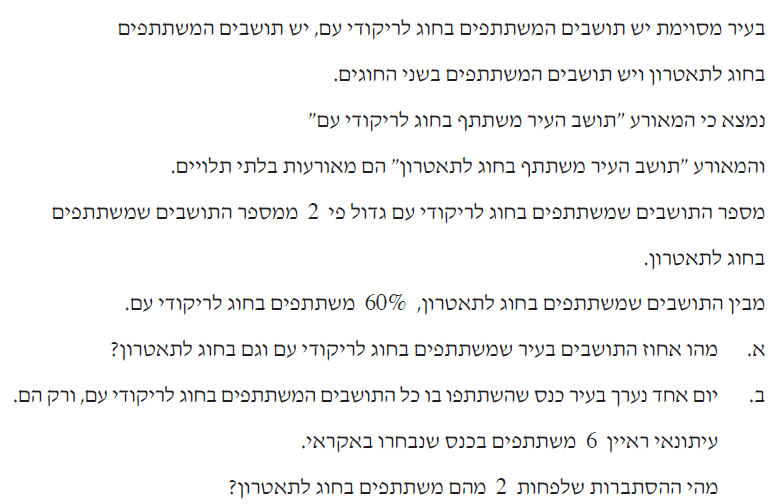
\includegraphics[width=.9\textwidth]{winter-2014-3}
%\end{center}

%%%%%%%%%%%%%%%%%%%%%%%%%%%%%%%%%%%%%%%%%%%%%%%%%%%%%%%%%%%%%%%%%%%

%
%\textbf{\R{
%קיץ תשע"ד, מועד א
%}}
%
%\begin{center}
%\selectlanguage{english}
%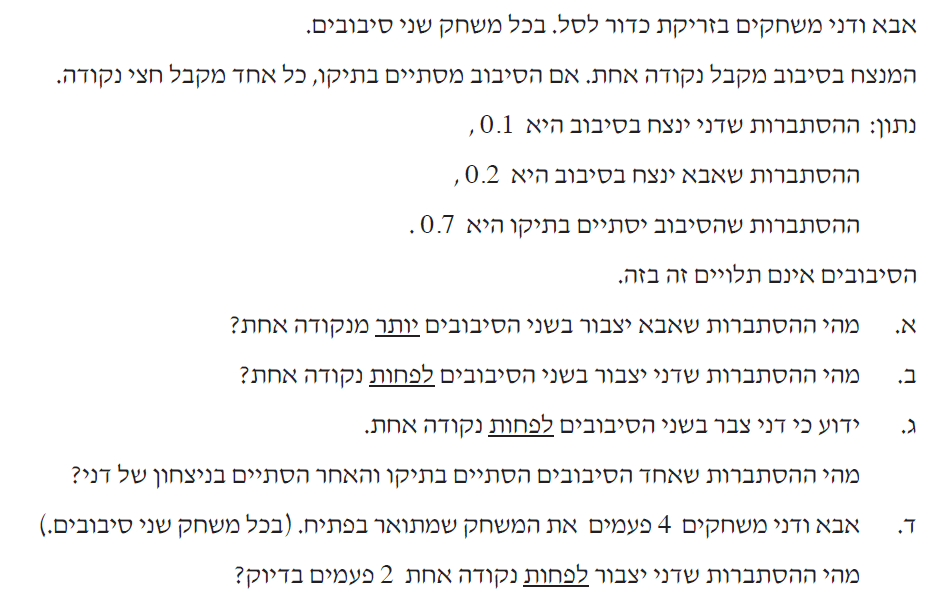
\includegraphics[width=.9\textwidth]{summer-2014a-3}
%\end{center}


%%%%%%%%%%%%%%%%%%%%%%%%%%%%%%%%%%%%%%%%%%%%%%%%%%%%%%%%%%%%%%%%%%%

%\textbf{\R{
%קיץ תשע"ד, מועד ב
%}}
%
%\begin{center}
%\selectlanguage{english}
%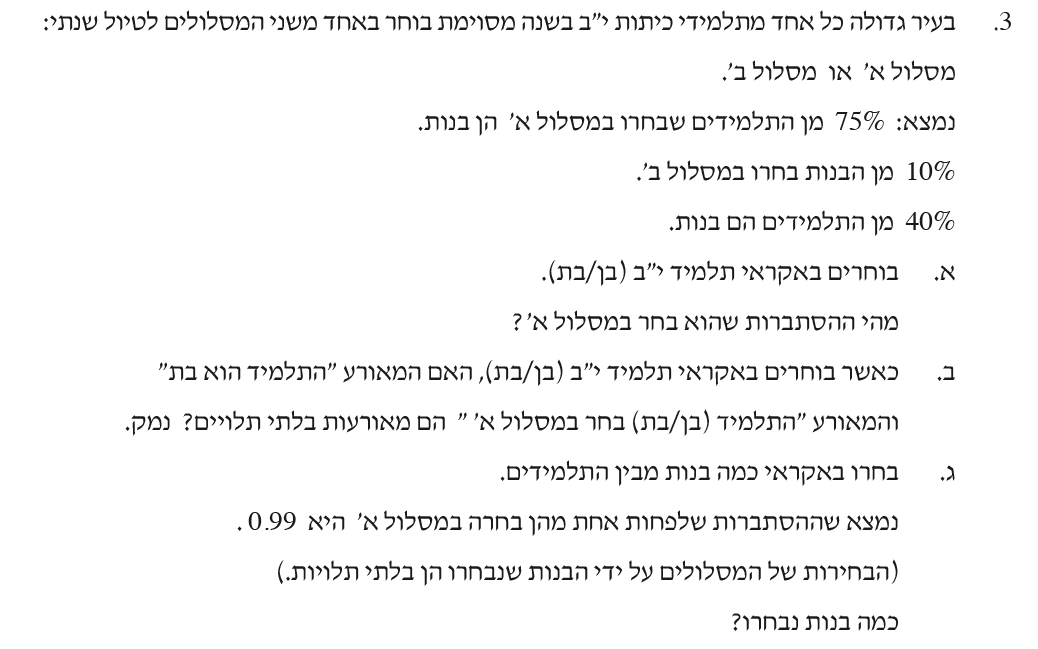
\includegraphics[width=.95\textwidth]{summer-2014b-3}
%\end{center}
%\vspace{-2ex}



%%%%%%%%%%%%%%%%%%%%%%%%%%%%%%%%%%%%%%%%%%%%%%%%%%%%%%%%%%%%%%%%%%%

%\textbf{\R{
%חורף תשע"ה
%}}
%
%\begin{center}
%\selectlanguage{english}
%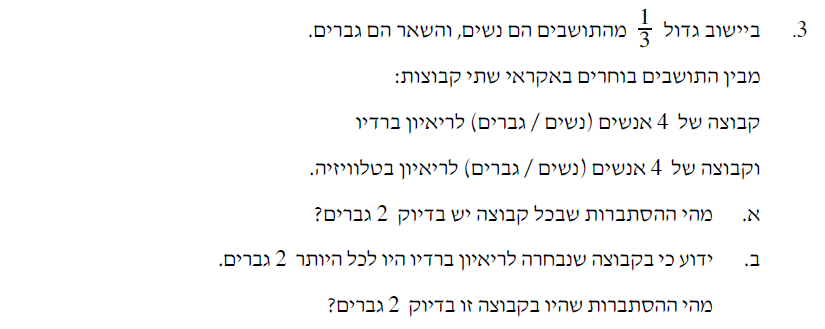
\includegraphics[width=.95\textwidth]{winter-2015-3}
%\end{center}


%%%%%%%%%%%%%%%%%%%%%%%%%%%%%%%%%%%%%%%%%%%%%%%%%%%%%%%%%%%%%%%%%%%
%
%\textbf{\R{
%קיץ תשע"ה, מועד א
%}}
%
%\begin{center}
%\selectlanguage{english}
%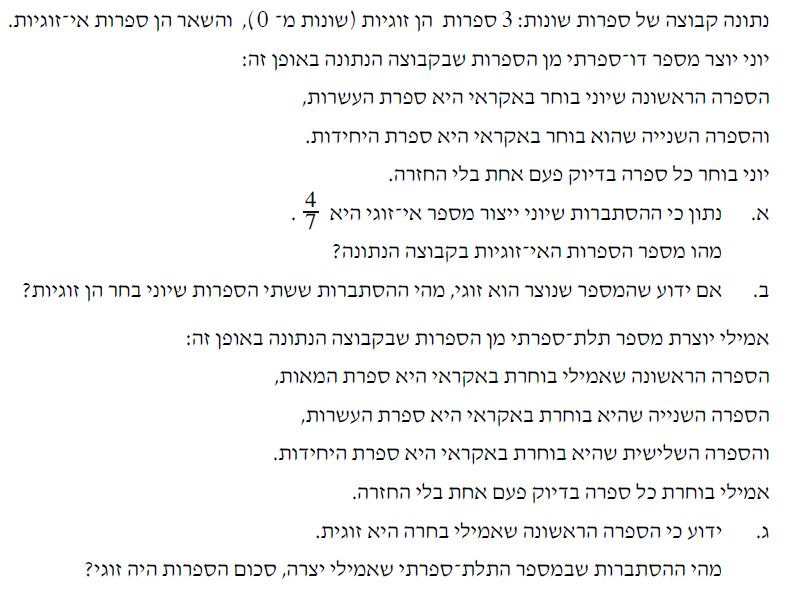
\includegraphics[width=.95\textwidth]{summer-2015a-3}
%\end{center}

%%%%%%%%%%%%%%%%%%%%%%%%%%%%%%%%%%%%%%%%%%%%%%%%%%%%%%%%%%%%%%%%%%%
%
%\textbf{\R{
%קיץ תשע"ה, מועד ב
%}}
%
%\begin{center}
%\selectlanguage{english}
%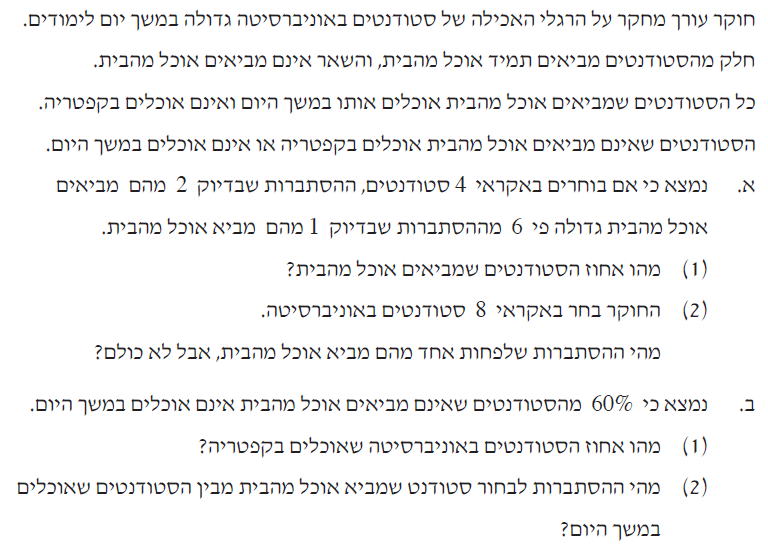
\includegraphics[width=.95\textwidth]{summer-2015b-3}
%\end{center}


%%%%%%%%%%%%%%%%%%%%%%%%%%%%%%%%%%%%%%%%%%%%%%%%%%%%%%%%%%%%%%%%%%%
%
%\textbf{\R{
%חורף תשע"ו
%}}
%
%\begin{center}
%\selectlanguage{english}
%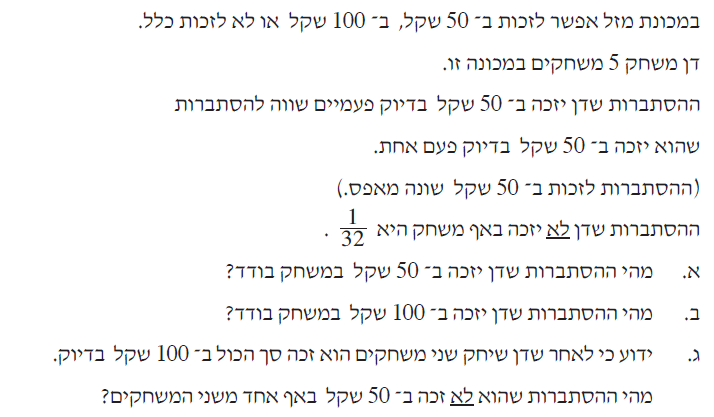
\includegraphics[width=.95\textwidth]{winter-2016-3}
%\end{center}


%%%%%%%%%%%%%%%%%%%%%%%%%%%%%%%%%%%%%%%%%%%%%%%%%%%%%%%%%%%%%%%%%%%
%
%\textbf{\R{
%קיץ תשע"ו, מועד א
%}}
%
%\begin{center}
%\selectlanguage{english}
%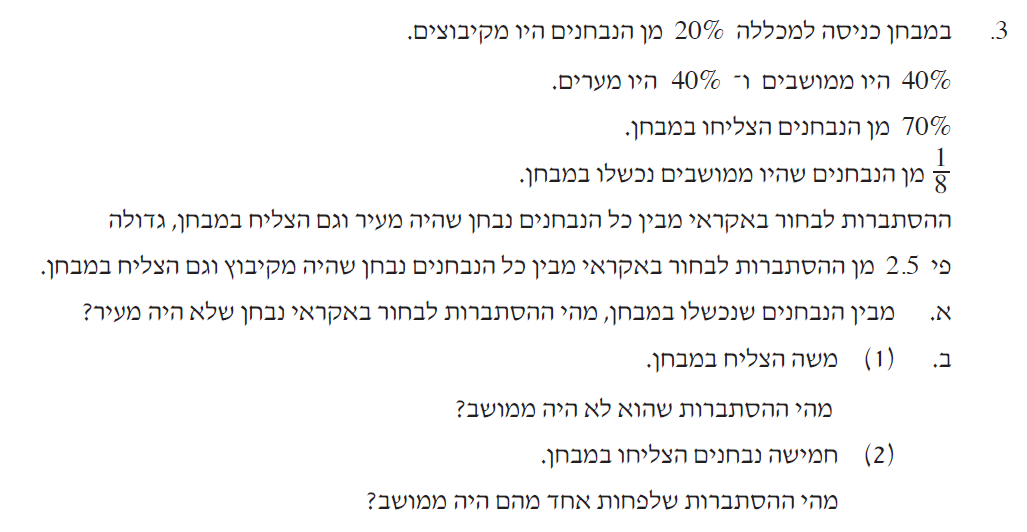
\includegraphics[width=.95\textwidth]{summer-2016a-3}
%\end{center}


%%%%%%%%%%%%%%%%%%%%%%%%%%%%%%%%%%%%%%%%%%%%%%%%%%%%%%%%%%%%%%%%%%%
%
%\textbf{\R{
%קיץ תשע"ו, מועד ב
%}}
%
%\begin{center}
%\selectlanguage{english}
%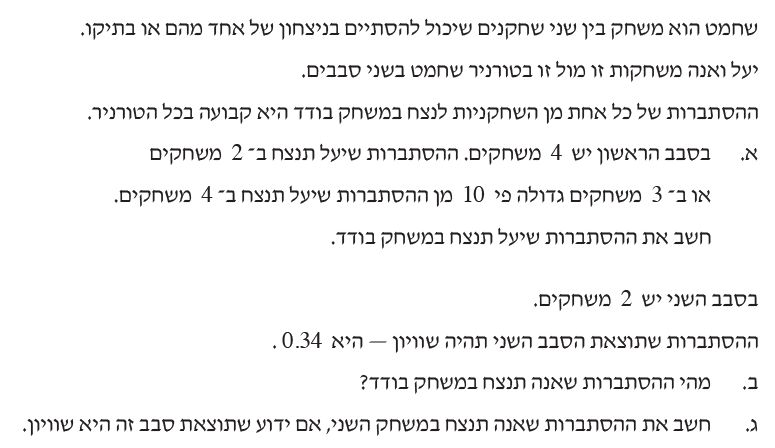
\includegraphics[width=.95\textwidth]{summer-2016b-3}
%\end{center}
%\vspace{-1ex}


%%%%%%%%%%%%%%%%%%%%%%%%%%%%%%%%%%%%%%%%%%%%%%%%%%%%%%%%%%%%%%%%%%%

\textbf{\R{
חורף תשע"ז
}}

\begin{center}
\selectlanguage{english}
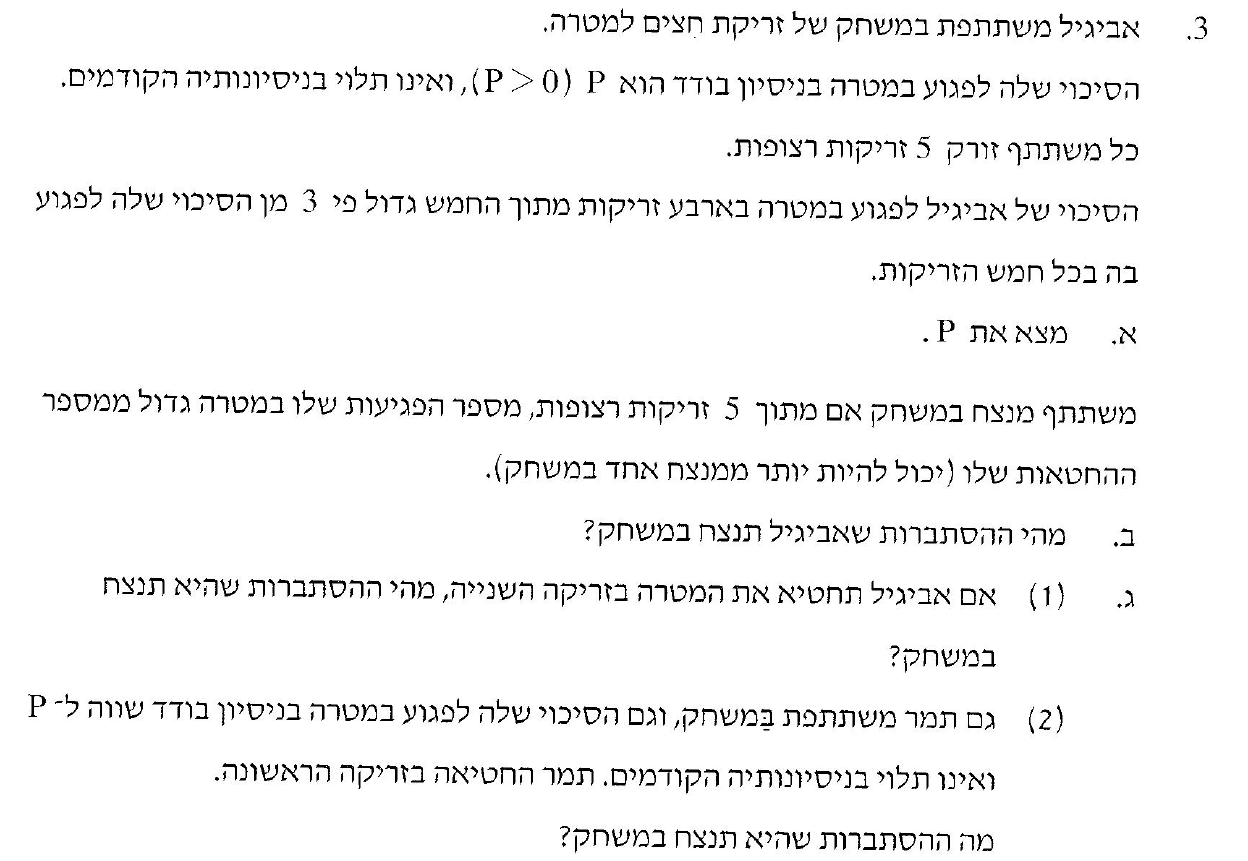
\includegraphics[width=.95\textwidth]{winter-2017-3.png}
\end{center}
\vspace{-1ex}

סעיף א. נשתמש בנוסחת ברנולי:
\begin{eqnarray*}
{5 \choose 4} p^4(1-p)^1 &=& 3p^5\\
5 (1-p) &=& 3p\\
p&=&\frac{5}{8}\,.
\end{eqnarray*}
סעיף ב. ההסתברות ל-%
$3,4,5$
פגיעות היא:
\[
{5 \choose 3}p^3(1-p)^2 + {5 \choose 4}p^4(1-p)^1 + {5 \choose 5}p^5(1-p)^0
\]
נציב את
$p=\frac{5}{8}$
ונקבל
$0.7248$.

סעיף ג 
$(1)$.
מצאתי שניסוח השאלה לא בהיר. אני פירשתי אותה: מה ההסתברות של
\textbf{האירוע}
"אביגיל מחטיאה בזריקה השנייה ופוגעת בשלוש או ארבע מהזריקות האחרות"? כותב הבחינה התכוון להסתברות מותנת: "%
\textbf{אם ידוע ש-}%
אביגיל החטיאה בזריקה השנייה, מה ההסתברות שהיא פוגעת בשלוש או ארבע מהזריקות האחרות"?
\[
\begin{array}{c}
P(1,3,4,5\ \textrm{\R{אביגיל פגעה בשלוש או ארבע מהזריקות}}/\textrm{\R{אביגיל החטיאה בזריקה השניה}}) =\\\\
\displaystyle\frac{P(1,3,4,5\ \textrm{\R{אביגיל החטיאה בזריקה השנייה ופגעה שלוש או ארבע מהזריקות}})}{P(\textrm{\R{אביגיל החטיאה בזריקה השניה}})} 
\end{array}
\]
שימו לב שהסתברות במנה היא נכונה לפי הפירוש שלי, וכדי לקבל את הפירוש הרשמי נחלק אותה בהסתברות להחטאה
$\frac{3}{8}$.
ההסתברות מורכבת משני גורמים. הראשון הוא ההסתברות של האירוע: "לא משנה מה יצאה מהזריקה הראשונה, הזריקה השניה החטיאה, ושלושת הזריקות האחרונות פגעו". הגורם השני הוא ההסתברות של האירוע: "הזריקה הראשונה פגעה, הזריקה השניה החטיאה, ושתיים מתוך שלושת הזריקות האחרונות פגעו":
\[
1\cdot \frac{3}{8} \cdot \left(\frac{5}{8}\right)^3 \quad + \quad
\frac{5}{8}\cdot \frac{3}{8} \cdot \left[{3\choose 2}\cdot\left(\frac{5}{8}\right)^2\cdot\frac{3}{8}\right] = \frac{375}{4096}+\frac{3375}{32768}=0.1945\,.
\]
נחלק ב-%
$\frac{3}{8}$
ונקבל את התשובה 
$0.5188$.

סעיף ג 
$(2)$.
שאלה זו זהה לשאלה בתת-סעיף הקודם. לא משנה איזו זריקה החטיאה, ההסתברות של האירוע היא 
$0.1945$
וכאשר מפרשים לפי הסתברות מותנית יש לחלק ב-%
$\frac{3}{8}$.
%%%%%%%%%%%%%%%%%%%%%%%%%%%%%%%%%%%%%%%%%%%%%%%%%%%%%%%%%%%%%%%%%%%

\textbf{\R{
קיץ תשע"ז, מועד א
}}

\begin{center}
\selectlanguage{english}
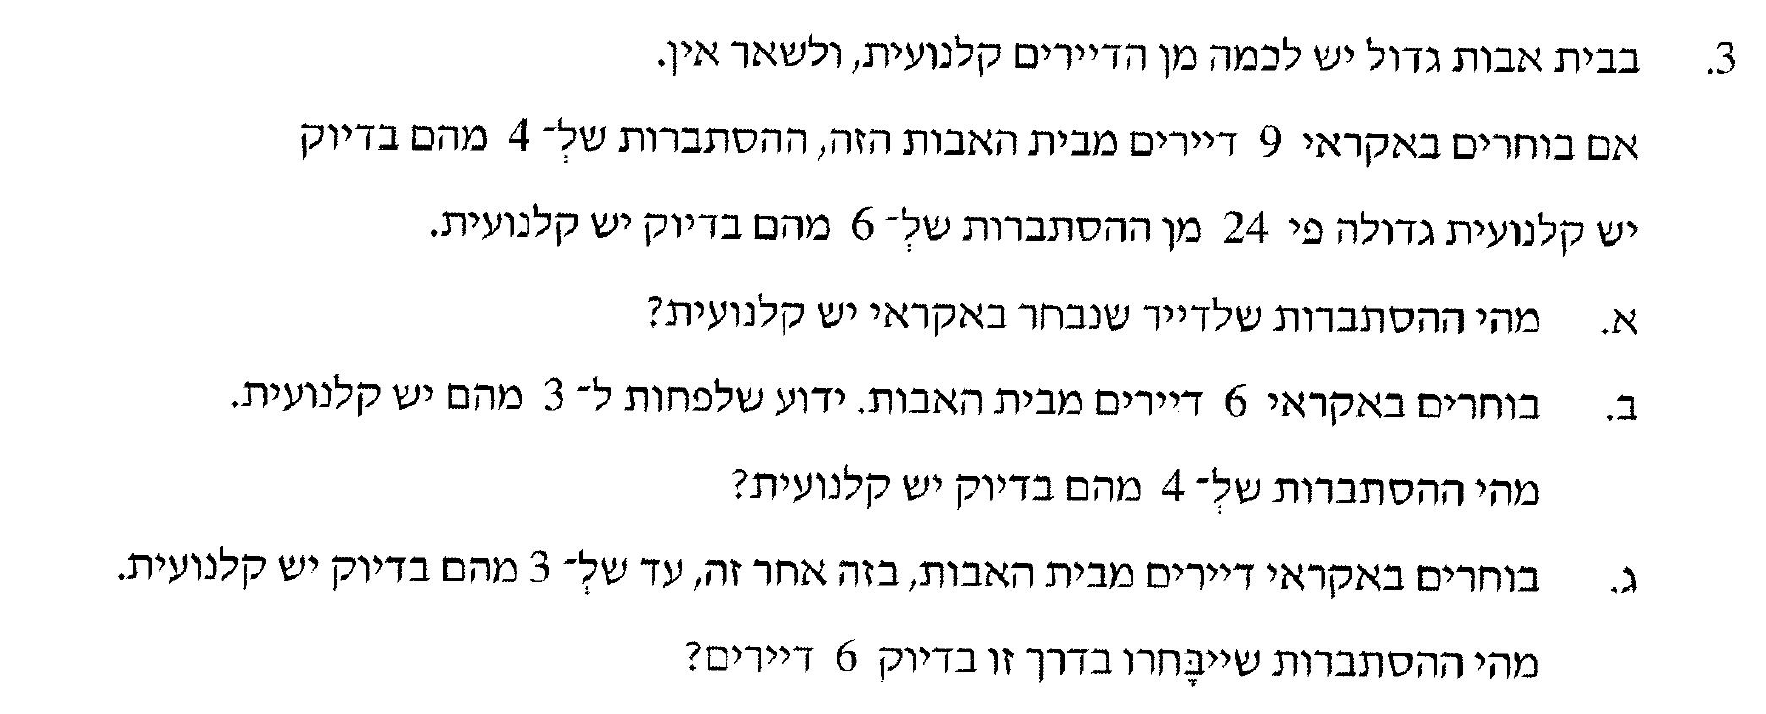
\includegraphics[width=.95\textwidth]{summer-2017a-3}
\end{center}

סעיף א. נסמן ב-%
$D$
את האירוע "דייר עם קלנועית" ואת ההסתברות של האירוע ב-%
$p$.
כאשר מבקשים
\textbf{בדיוק}
את כמות ה-"הצלחות" 
$k$
מ-%
$n$
בחירות אקראיות, נשתמש בנוסחת ברנולי:
\[
P_n(k)={n\choose k} p^k (1-p)^{n-k}\,,
\]
כאן:
\[
P_9(4)={9\choose 4} p^4 (1-p)^5=24P_9(6)=24 {9\choose 6} p^6 (1-p)^3\,.
\]
נפשט את המשוואה ונקבל משוואה ריבונית:
\[
15p^2+2p-1=0\,,
\]
שיש לה שני פתרונות
$p=\frac{1}{5},-\frac{1}{3}$.
ההסתברות לא יכולה להיות שלילית ולכן התשובה היא 
$p=\frac{1}{5}$.

סעיף ב. המילה
\textbf{ידוע}
מכוונת אותנו להסתברות מותנת:
\[
P(D=4/D\ge3) = \frac{P(D=4\cap D\ge 3)}{P(D\ge 3)}\,.
\]
כאשר יש חפיפה בין ביטויים בחיתוך אפשר לפשט אותו. ברור שאם ערך גדול או שווה
$3$
\textbf{וגם}
שווה ל-%
$4$,
אז הוא שווה ל-%
$4$.
\[
P(D=4/D\ge3) =\frac{P(D=4)}{P(D\ge 3)}\,.
\]
את הערך של
$P(D=4)$
נחשב לפי נוסחת ברנולי:
\[
{6\choose 4}\cdot 0.2^4 \cdot 0.8^2= 0.01536\,.
\]
את הערך של
$P(D\ge 3)$
אפשר לחשב בשתי דרכים, בצורה ישירה או כאחד פחות המשלים:
\begin{eqnarray*}
P(D\ge 3) &=& P(D=3) + P(D=4) + P(D=5) + P(D=6)\\
1-P(D\ge 3) &=& 1- P(D<3)=1-(\,P(D=0) + P(D=1) + P(D=2)\,)\,.
\end{eqnarray*}
נבחר את האפשרות השנייה כי יש פחות גורמים בביטוי:
\[
1-0.8^6-{6\choose 1}\cdot 0.2^1\cdot 0.8^5 - {6 \choose 2}\cdot 0.2^2\cdot 0.8^4=0.099\,,
\]
והתשובה היא
$\displaystyle\frac{0.01536}{0.099}=0.15534$.

סעיף ג. מפסיקים את הבחירה כאשר יש בדיוק שלושה דיירים עם קלנועית. מכאן שהבחירה 
\textbf{האחרונה} 
היא "הצלחה" ויש שתי "הצלחות" נוספות בחמשת הבחירות הקודמות:
\[
\overbrace{\pm\;\pm\;\pm\;\pm\;\pm}^{2/5}\quad\quad \overbrace{+}^{1/1}\,.
\]
התשובה מתקבלת מנוסחת ברנולי לבחירות הראשונות כפול ההסתברות
$p$
לבחירה האחרונה:
\[
{5\choose 2}\cdot 0.2^2 \cdot 0.8^3 \;\cdot\; 0.2=0.04096\,.
\]

%%%%%%%%%%%%%%%%%%%%%%%%%%%%%%%%%%%%%%%%%%%%%%%%%%%%%%%%%%%%%%%%%%%

\textbf{\R{
קיץ תשע"ז, מועד ב
}}

\begin{center}
\selectlanguage{english}
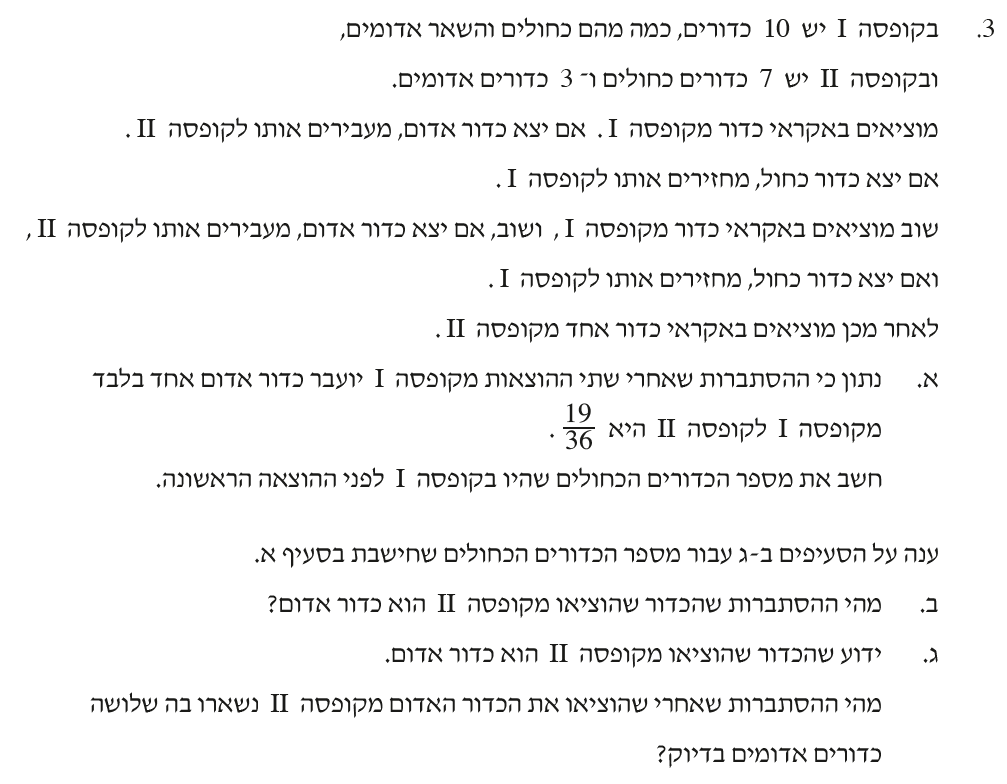
\includegraphics[width=.95\textwidth]{summer-2017b-3}
\end{center}

הביטוי
\textbf{מוציאים באקראי}
ואחר כך
\textbf{שוב מוציאים באקראי}
מכוון אותנו לשימוש בעץ כדי לתאר את הבחירה הסדרתית. נסמן ב-%
\textsf{A}
את מספר הכדורים האדומים בקופסה 
\textsf{I}.

באיור להלן, בכל צומת רשום שני זוגות של מספרים: מספר הכדורים האדומים ומספר הכדורים הכחולים בקופסה
\textsf{I},
ומתחתיו מספר הכדורים האדומים ומספר הכדורים הכחולים בקופסה
\textsf{II}.
הכוכבית מסמנת את שתי האפשרויות בהן הוצאנו כדור אדום אחד בדיוק מקופסה
\textsf{I}.
שימו לב שמספר הכדורים הכחולים בכל אחת המקופסאות לא משתנה.

\selectlanguage{english}
\begin{center}
\begin{tikzpicture}
[grow=right,
level 1/.append style={font=\sffamily,text width=2cm,level distance=3.5cm,sibling distance=10em},
level 2/.append style={font=\sffamily,text width=2.5cm,level distance=4.5cm,sibling distance=5em}]
\node[font=\sffamily,text width=2cm] {(A,10-A)\\(3,7)} % root
child {
  node {(A,10-A)\\(3,7)}
    child {
      node {(A,10-A)\\(3,7)}
      edge from parent node[below] {\R{כחול} I}
    }
    child {
      node {(A-1,10-A)\ *\\(4,7)}
      edge from parent node[above] {\R{אדום} I}
    }
    edge from parent node[below] {\R{כחול} I}
}
child { 
  node {(A-1,10-A)\\(4,7)}
    child {
      node {(A-1,10-A)\ *\\(4,7)}
      edge from parent node[below] {\R{כחול} I}
    }
    child {
      node {(A-2,10-A)\\(5,7)}
      edge from parent node[above] {\R{אדום} I}
    }
    edge from parent node[above] {\R{אדום} I}
};
\end{tikzpicture}
\end{center}
\selectlanguage{hebrew}

נשווה את הסתברות הנתונה לשתי האפשרויות לסכום ההסתברויות של שני המסלולים:
\[
\frac{A}{10}\cdot\frac{10-A}{9} + \frac{10-A}{10}\cdot\frac{A}{10} = \frac{19}{36}\,.
\]
נפשט ונקבל משוואה ריבועית 
$x^2-10a+25=0$
שיש לה פתרון אחד
$a=$,
שהוא גם מספר הכדורים הכחולים  וגם מספר הכדורים האדומים בקופסה
\textsf{I}.

סעיף ב. עבור כל מצב סופי, ההסתברות להוציא כדור אדום מקופסה
\textsf{II}
הוא מספר הכדורים האדומים בקופסה לחלק למספר הכדורים בקופסה:
\[
\frac{5}{5+7},\; \frac{4}{4+7},\; \frac{4}{4+7},\; \frac{3}{3+7}\,.
\]
כדי לקבל את ההסתברות לכל המצבים, נסכם את ההסתברויות אלו לאחר הכפלתן בהסתברות להגיע למצב:
\[
\frac{5}{10}\cdot\frac{4}{9}\cdot\frac{5}{12}+\frac{5}{10}\cdot\frac{5}{9}\cdot\frac{4}{11}+\frac{5}{10}\cdot\frac{5}{10}\cdot\frac{4}{11}+\frac{5}{10}\cdot\frac{5}{10}\cdot\frac{3}{10}=0.3595\,.
\]

סעיף ג. המילה 
\textbf{ידוע}
מכוון להסתברות מותנת. אם רואים באיור שיישארו שלושה כדורים אדומים רק אם היו אברעה כדורים אדומים לפני הבחירה, כלומר, אותם שני מצבים המסומנים כוכבית.
\[
\begin{array}{c}
P(\textrm{II \R{נשארו שלושה אדומים בקופסה}}/\textrm{II \R{הוציאו כדור אדום מקופסה}}) =\\\\
\displaystyle\frac{P(\textrm{II \R{נשארו שלושה אדומים בקופסה}} \cap \textrm{II \R{הוציאו כדיר אדום מקופסה}})}{P(\textrm{II \R{הוציאו כדור אדום מקופסה}})}
\end{array}
\]
ההסדברות במנה היא ההסתברות )הנתונה!( שנגיע לאחד המצבים המסומנים בכוכבית כפול ההסתברות לבחור אדום מקופסה 
\textsf{II},
וההסתברות במכנה חישבנו בסעיף ב. התשובה היא:
\[
\frac{\displaystyle\frac{19}{36}\cdot\frac{4}{11}}{0.3595}=0.53385\,.
\]

%%%%%%%%%%%%%%%%%%%%%%%%%%%%%%%%%%%%%%%%%%%%%%%%%%%%%%%%%%%%%%%%%%%


\textbf{\R{
חורף תשע"ח
}}

\begin{center}
\selectlanguage{english}
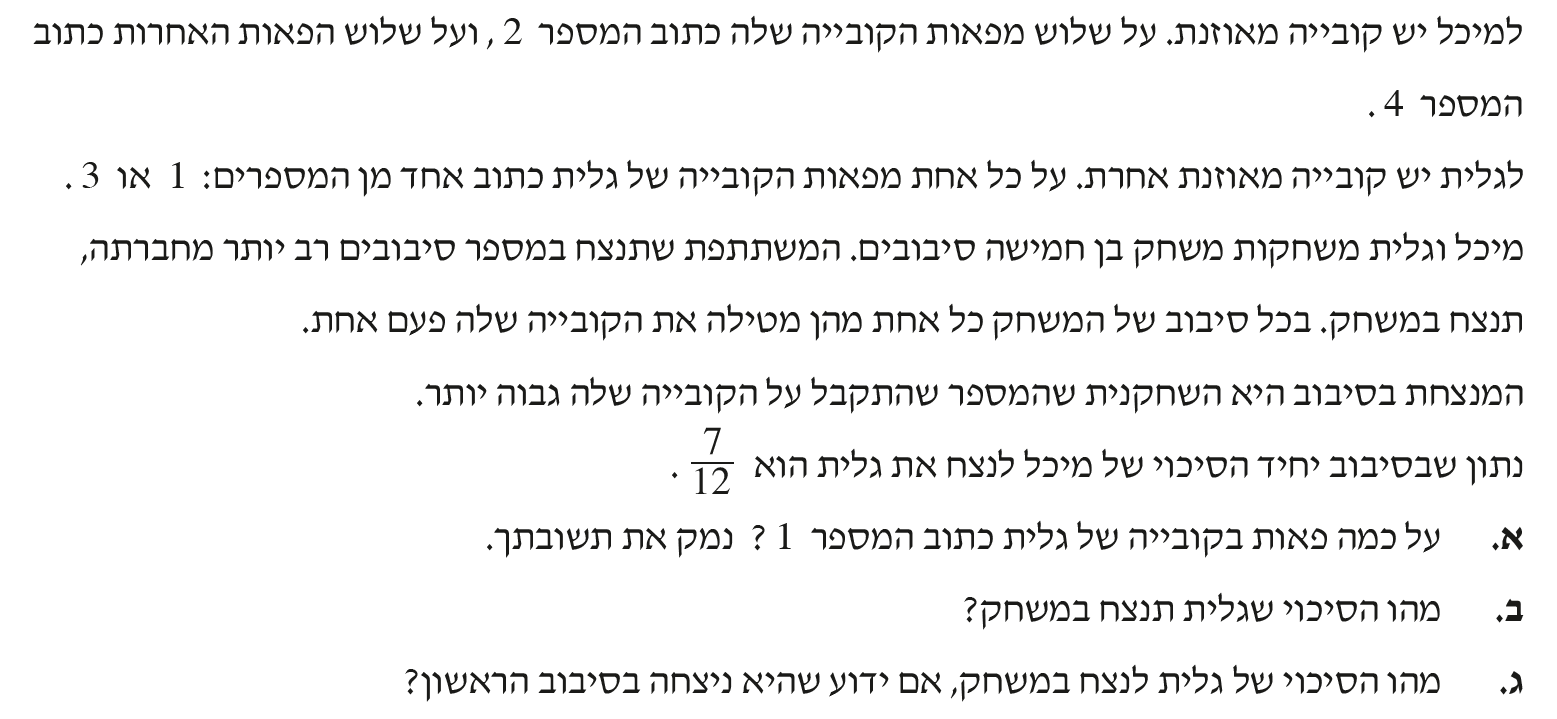
\includegraphics[width=\textwidth]{winter-2018-3}
\end{center}

סעיף א. נתון הסיכוי של מיכל לנצח שיקרה אם מיכל מטילה 
$4$
)לא משנה מה גלית מטילה(, או אם מיכל מטילה 
$2$
וגלית מטילה
$1$.
נסמן ב-%
$n$
את המספר הפאות של הקוביה של גלית שכתוב עליהן
$1$.
המשוואה לניצחון של מיכל היא:
\[
\frac{3}{6}\cdot 1 + \frac{3}{6}\cdot \frac{n}{6}=\frac{7}{12}\,.
\]
הפתרון של המשוואה הוא
$n=1$.

סעיף ב. גלית תנצח אם היא תנצח ב-%
$3,4,5$
סיבובים. לפי נוסחת ברנולי ההסתברות היא:
\[
{5\choose 3}\left(\frac{5}{12}\right)^3\left(\frac{7}{12}\right)^2+{5\choose 4}\left(\frac{5}{12}\right)^4\left(\frac{7}{12}\right)^1+{5\choose 5}\left(\frac{5}{12}\right)^5\left(\frac{7}{12}\right)^0=0.3466\,.
\]

סעיף ג. השאלה דומה לשאלה בבחינה של
\textbf{חורף תשע"ז}.
את החישוב נעשה בדרך שונה המשתמשת בעובדה ההטלות הקוביה בלתי תלויות אחת מהשנייה:
\[
\begin{array}{c}
P(\textrm{\R{גלית תנצח}}\ /\textrm{\R{גלית ניצחה בסיבוב הראשון}}) =\\\\
\displaystyle\frac{P(\textrm{\R{גלית תנצח בשנים מתוך ארבעה סיבובים אחרונים}})\cdot P(\textrm{\R{גלית ניצחה בסיבוב הראשון}})}{P(\textrm{\R{גלית ניצחה בסיבוב הראשון}})}\,.
\end{array}
\]
לאחר צימצום, התשובה היא:
\[
{4 \choose 4}\left(\frac{5}{12}\right)^4 \left(\frac{7}{12}\right)^0+
{4 \choose 3}\left(\frac{5}{12}\right)^3 \left(\frac{7}{12}\right)^1+
{4 \choose 2}\left(\frac{5}{12}\right)^2 \left(\frac{7}{12}\right)^2
=0.5534\,.
\]



%%%%%%%%%%%%%%%%%%%%%%%%%%%%%%%%%%%%%%%%%%%%%%%%%%%%%%%%%%%%%%%%%%%

\textbf{\R{
קיץ תשע"ח, מועד א
}}

\begin{center}
\selectlanguage{english}
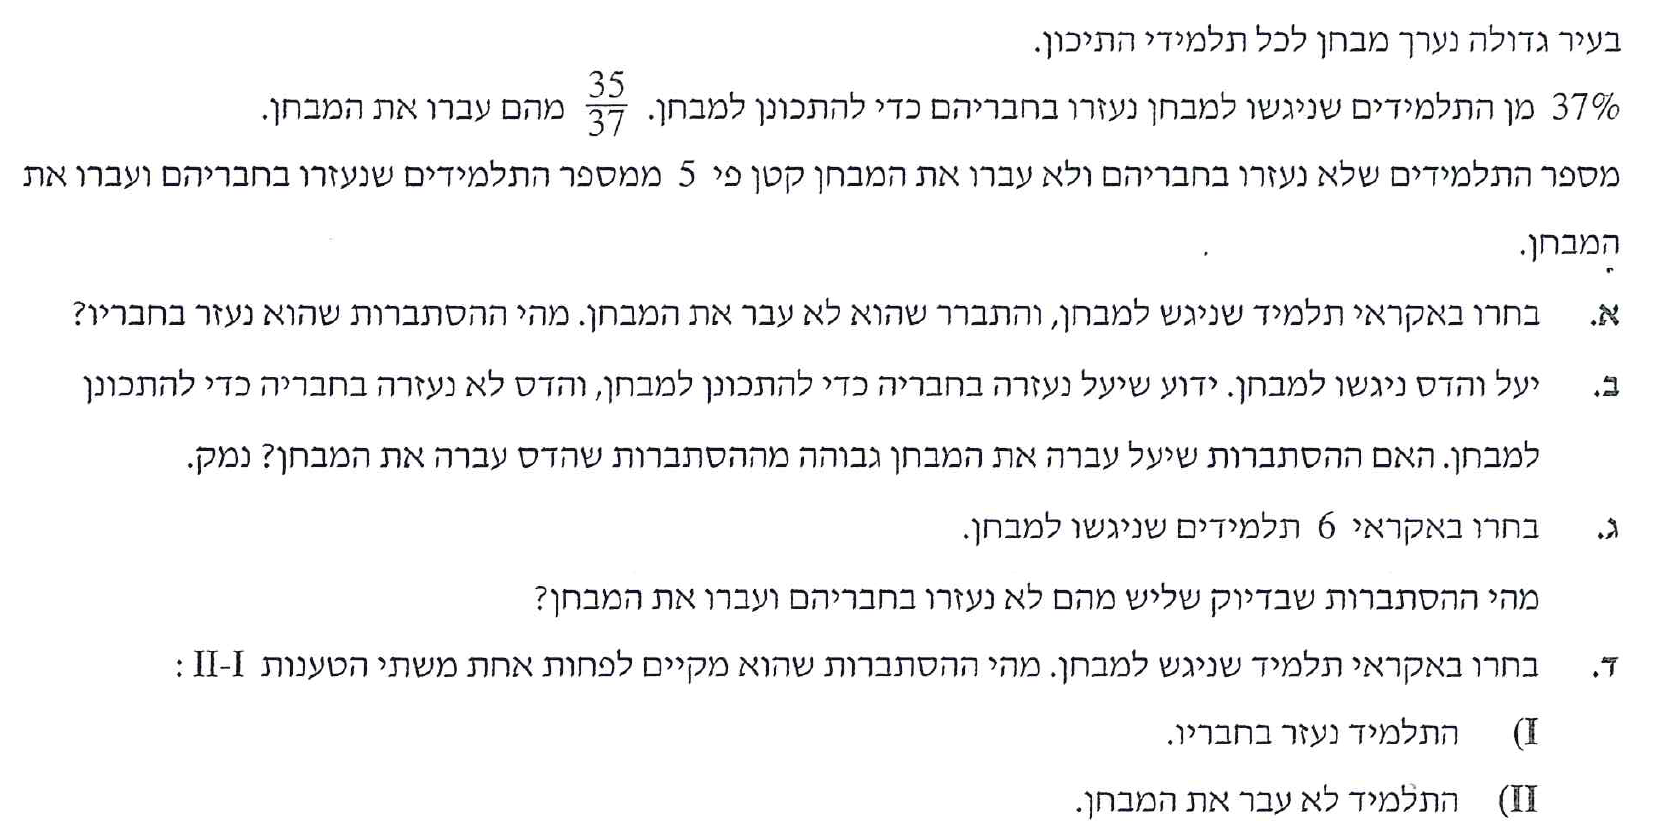
\includegraphics[width=\textwidth]{summer-2018a-3}
\end{center}
כאשר שני אירועים שונים מופיעים בשאלה נבנה טבלה כדי להציג את ההסתברות של כל אירוע וההסתברות של כל חיתוך של האירועים.

נסמן ב-%
$N$
את התלמידים שנעזרו בחבריהם, וב-%
$A$
את התלמידים שעברו את המבחן. נתון ש-%
$P(N)=0.37$,
וש-%
$P(A/N)$.
נחשב:
\[
P(A/N) = \frac{P(N\cap A)}{P(N)} = \frac{P(N\cap A)}{0.37}=\frac{35}{37},\quad\quad\quad P(N\cap A)=0.35\,.
\]
עד כאן הטבלה של ההסתברויות היא:
\begin{center}
\selectlanguage{english}
\begin{tikzpicture}[scale=1.25]
\draw (0,0) grid (3,3);
\node at (2.5,3.3) {$\bm{A}$};
\node at (1.5,3.3) {$\bover{A}$};
\node at (3.3,2.5) {$\bm{N}$};
\node at (3.3,1.5) {$\bover{N}$};
\node at (2.5,2.5) {$0.35$};
\node at (0.5,2.5) {$0.37$};
\node at (1.5,2.5) {$0.02$};
\node at (0.5,1.5) {$0.63$};
\node at (0.5,0.5) {$1.0$};
\end{tikzpicture}
\end{center}
בהמשך נתון ש-%
\[
P(\overline{N}\cap\overline{A})=\frac{P(N\cap A)}{5}=\frac{0.35}{5}=0.07\,,
\]
וניתן להשלים את הטבלה:
\begin{center}
\selectlanguage{english}
\begin{tikzpicture}[scale=1.25]
\draw (0,0) grid (3,3);
\node at (2.5,3.3) {$\bm{A}$};
\node at (1.5,3.3) {$\bover{A}$};
\node at (3.3,2.5) {$\bm{N}$};
\node at (3.3,1.5) {$\bover{N}$};
\node at (2.5,2.5) {$0.35$};
\node at (0.5,2.5) {$0.37$};
\node at (1.5,2.5) {$0.02$};
\node at (0.5,1.5) {$0.63$};
\node at (0.5,0.5) {$1.0$};
\node at (1.5,0.5) {$0.09$};
\node at (2.5,0.5) {$0.91$};
\node at (1.5,1.5) {$0.07$};
\node at (2.5,1.5) {$0.56$};
\end{tikzpicture}
\end{center}
בעזרת הטבלה ניתן למצוא את התשובות לשאלות.

סעיף א.
\[
P(N/\overline{A})=\frac{N\cap \overline{A}}{\overline{A}}=\frac{0.02}{0.09}=\frac{2}{9}\,.
\]
סעיף ב. עבור יעל:
\[
P(A/N)=\frac{A \cap N}{N}=\frac{0.35}{0.37}=0.9459\,,
\]
ועבור הדס:
\[
P(A/\overline{N})=\frac{A\cap \overline{N}}{\overline{N}}=\frac{0.56}{0.63}=0.8889\,.
\]
ליעל סיכוי טוב יותר לעבור את המבחן.

\[
P(N/\overline{A})=\frac{N\cap \overline{A}}{\overline{A}}=\frac{0.02}{0.09}=\frac{2}{9}\,.
\]
סעיף ג. שליש משש הוא שניים. )שימו לב לא ליפול למלכודת ולקרוא "שלושה" במקום "שליש"!( החישוב הוא לפי נוסחת ברנולי כאשר הערך של
$P(\overline{N}\cap A)$
נמצא בטבלה:
\[
{6 \choose 2}(0.56)^2 (0.44)^4=0.1763\,.
\]

סעיף ד. הניסוח "%
\textbf{לפחות אחת}
משתי הטענות I,II" אומר שהאירוע קורה אם קורה אחד מהאירועים I, II
\textbf{או שניהם}.
באיור להלן שני המעגלים מייצגים את שני האירועים I ו-II. האירוע "לחות אחד משניהם" מיוצג על ידי כל השטח המקווקו.
\begin{center}
\selectlanguage{english}
\begin{tikzpicture}
\begin{scope}
\clip[draw] (0,0) circle[radius=2];
\foreach \y in {-1.5,-1,-.5,0,.5,1,1.5}
  \draw (-2,\y) -- (2,\y);
\end{scope}
\begin{scope}
\clip[draw] (2.5,0) circle[radius=2];
\foreach \x in {1,1.5,2,2.5,3,3.5,4}
  \draw (\x,-2) -- (\x,2);
\end{scope}
\node at (-2,2.5) {$I$};
\node at (4.5,2.5) {$II$};
\node at (1.25,2.5) {$I\cap II$};
\node at (-3.5,.2) {$I/ II$};
\node at (6,.2) {$II/ I$};
\draw[->] (1.25,2.2) -- ++(0,-1);
\draw[->] (-3,.2) -- ++(1.7,0);
\draw[->] (5.5,.2) -- ++(-1.7,0);
\end{tikzpicture}
\end{center}
 יש שתי דרכים לחשב את ההסתברות:
\begin{eqnarray*}
P(I \cup II) &=& P(I) + P(II) - P(I \cap II)\\
P(I \cup II) &=& P(I/ II) + P(II/ I) - P(I \cap II)\,.
\end{eqnarray*}
בדרך הראשונה אנו לוקחים את סכום ההסתברויות של שני האירועים ואז מחסירים את ההסתברות של האירוע המשותף כי ספרנו אותו פעמיים, פעם כחלק מהאירוע I ופעם כחלק מהאירוע II. בדרך השניה אנו סופרים כל חלק מהאירוע השותף בנפרד.

את ההסתברויות לחישוב 
$P(N\cup\overline{A})$
ניקח מהטבלה, ואין הבדל מהותי בין שתי הדרכים. הדרך הראשונה מופיעה מימין והדרך השניה משמאל:
\begin{center}
\selectlanguage{english}
\begin{tikzpicture}[scale=1.25]
\begin{scope}
\draw (0,0) grid (3,3);
\node at (2.5,3.3) {$\bm{A}$};
\node at (1.5,3.3) {$\bover{A}$};
\node at (3.3,2.5) {$\bm{N}$};
\node at (3.3,1.5) {$\bover{N}$};
\node at (2.5,2.5) {$0.35$};
\node at (0.5,2.5) {$0.37$};
\node at (1.5,2.5) {$0.02$};
\node at (0.5,1.5) {$0.63$};
\node at (0.5,0.5) {$1.0$};
\node at (1.5,0.5) {$0.09$};
\node at (2.5,0.5) {$0.91$};
\node at (1.5,1.5) {$0.07$};
\node at (2.5,1.5) {$0.56$};
\draw[ultra thick] (2,2) rectangle +(1,1);
\draw[ultra thick] (1,1) rectangle +(1,1);
\draw[ultra thick] (1,2) rectangle +(1,1);
\end{scope}
\begin{scope}[xshift=6cm]
\draw (0,0) grid (3,3);
\node at (2.5,3.3) {$\bm{A}$};
\node at (1.5,3.3) {$\bover{A}$};
\node at (3.3,2.5) {$\bm{N}$};
\node at (3.3,1.5) {$\bover{N}$};
\node at (2.5,2.5) {$0.35$};
\node at (0.5,2.5) {$0.37$};
\node at (1.5,2.5) {$0.02$};
\node at (0.5,1.5) {$0.63$};
\node at (0.5,0.5) {$1.0$};
\node at (1.5,0.5) {$0.09$};
\node at (2.5,0.5) {$0.91$};
\node at (1.5,1.5) {$0.07$};
\node at (2.5,1.5) {$0.56$};
\draw[ultra thick] (0,2) rectangle +(1,1);
\draw[ultra thick] (1,0) rectangle +(1,1);
\draw[ultra thick] (1,2) rectangle +(1,1);
\end{scope}
\end{tikzpicture}
\end{center}
בשתי הדרכים מקבלים אותה תוצאה:
\begin{eqnarray*}
P(N\cup\overline{A})&=&P(N) + P(\overline{A}) - P(N\cap\overline{A}) = 0.37+0.09-0.02=0.44\\
P(N\cup\overline{A})&=&P(N/\overline{A}) + P(\overline{A}/ N) + P(N\cap\overline{A}) = 0.35+0.07+0.02=0.44\,.
\end{eqnarray*}


%%%%%%%%%%%%%%%%%%%%%%%%%%%%%%%%%%%%%%%%%%%%%%%%%%%%%%%%%%%%%%%%%%%

\textbf{\R{
קיץ תשע"ח, מועד ב
}}

\begin{center}
\selectlanguage{english}
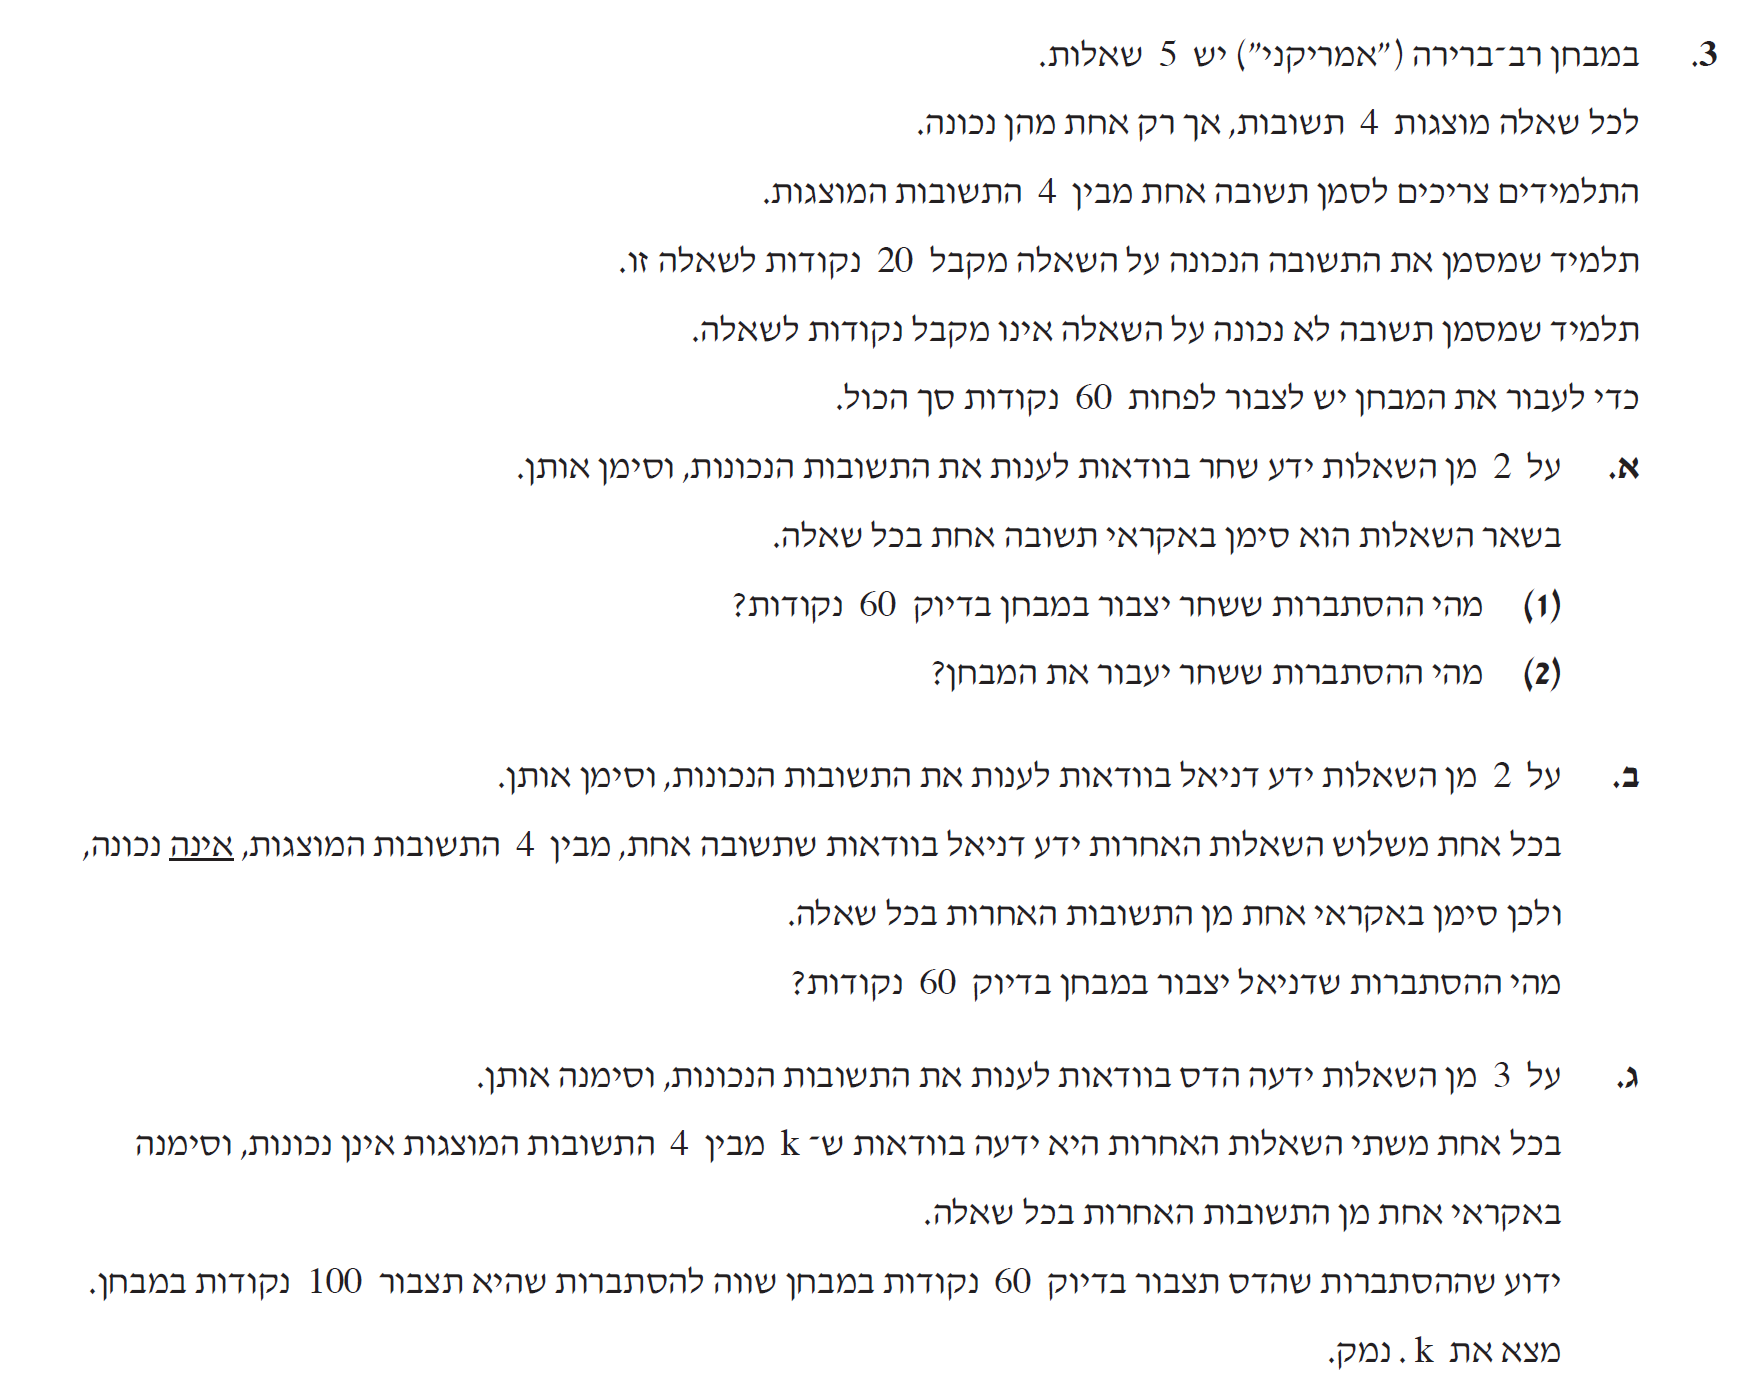
\includegraphics[width=\textwidth]{summer-2018b-3}
\end{center}

סעיף א
$(1)$.
שחר ידע שהוא ענה על שתי שאלות ולכן כדי לקבל ציון
$60$
עליו לענות על 
\textbf{בדיוק אחת}
משלושת השאלות האחרות, שניתן לחישוב על ידי נוסחת ברנולי:
\[
{3 \choose 1}\left(\frac{1}{4}\right)\left(\frac{3}{4}\right)^2=\frac{27}{64}\,.
\]
סעיף א
$(2)$.
כדי לעבור את המבחן עליו לצבור
\textbf{לפחות שלוש}
תשובות נכונות. לכן, עלינה להוסיף את ההסבתרויות של ארבע וחמש תשובות נכונות:
\[
\frac{27}{64}+{3 \choose 2}\left(\frac{1}{4}\right)^2\left(\frac{3}{4}\right)^1+{3 \choose 3}\left(\frac{1}{4}\right)^3\left(\frac{3}{4}\right)^0=\frac{37}{64}\,.
\]
סעיף ב.
כמו שחר, דניאל צירך לענות נכון על שאלה אחת 
\textbf{בדיוק}
מתוך שלושת השאלות הנותרות. דניאל יודע שתשובה אחת מתוך ארבע לא נכונה, לכן ההסתברות שהוא יענה נכון על השאלה היא
$\frac{1}{3}$.
לפי נוסחת ברנולי:
\[
{3 \choose 1}\left(\frac{1}{3}\right)\left(\frac{2}{3}\right)^2=\frac{4}{9}\,.
\]
סעיף ג. אם הדס יודעת ש-%
$k$
מתוך 
$4$
תשובות לא נכונות, מספר התשובות שמהן היא בוחרת באקראי הוא
$4-k$.
הסיכוי לענות תשובה נכונה היא
$\frac{1}{4-k}$
וסיכוי לענות תשובה לא נכונה היא
$\frac{4-k-1}{4-k}$
כי אם תשובה אחת מתוך 
$4-k$
נכונה, כל שאר התשובות לא נכונות.

כדי לקבל ציון 
$100$
ברור שהיא צריכה לבחור תשובות נכונות לשתי השאלות הנותרות. כדי לקבל ציון 
\textbf{בדיוק}
$60$
עליה לבחר תשובות לא נכונות לשתי השאלות הנותרות. החישוב הוא פשוט לפי מכפלת הסתברויות של אירועים בלתי תלויים:
\begin{eqnarray*}
\left(\frac{1}{4-k}\right)^2 &=&\left(\frac{4-k-1}{4-k}\right)^2\\
(3-k)^2&=&1\\
k^2-6k+8&=& 0\,.
\end{eqnarray*}
הפתרונות של המשוואה הם 
$k=2,k=4$
אבל נתון ש-"אחת מהן נכונה", לכן הפתרון האפשרי היחיד הוא
$k=2$.

%%%%%%%%%%%%%%%%%%%%%%%%%%%%%%%%%%%%%%%%%%%%%%%%%%%%%%%%%%%%%%%%%%%

\newpage

\begin{center}
\textbf{סיכום}
\end{center}

\begin{itemize}
\item
\textbf{קרא בזהירות את השאלה}.

\item
המילה 
\textbf{בדיוק}
מכוונת לחישוב אחד של נוסחת ברנולי, כי נתון כמה "הצלחות" צריכות להיות וגם כמה "כשלונות". מקרה מעניין נמצא בבחינה של
\textbf{קיץ תשע"ח ב}
כאשר נתון שההסתברות לקבל 
$60$
שווה להתברות לקבל
$100$.
נתון גם שיש שלוש הצלחות מתוך חמש, אז ההסתברות לקבל שני "כשלונות" צריכה להיות שווה להסתברות לקבל שתי "הצלחות".

\item
שימו לב לניסוחים המכוונים להסתברות מותנת:
\begin{itemize}
\item
בבחינה של
\textbf{חורף תשע"ז}
סעיף ג
$(1)$
כתוב "%
\textbf{אם} $\ldots$ ,
\textbf{מהי ההסתברות} $\ldots$".
לא לגמרי ברור שלמילה אם יש משמעות של אם ידוע, אבל זאת הכוונה.
\item
הניסוח בבחינה של
\textbf{קיץ תשע"ז א}
סעיף ב ברור יותר:
\textbf{אם} $\ldots$ ,
\textbf{מהי ההסתברות} $\ldots$".
\end{itemize}

\item
כאשר יש חיתוך בחישוב של הסתברות מותנת, לעתים קרובות ניתן לפשט את החישב. בבחינה של
\textbf{קיץ תשע"ז א}
יש לחשב
$P(D=4\cap D\ge 3)$,
אבל אם ערך גדול או שווה
$3$
\textbf{וגם}
שווה ל-%
$4$,
אז הוא שווה ל-%
$4$, 
ולכן מספיק לחשב
$P(D=4)$.

\item
 בבחינה של
\textbf{קיץ תשע"ז א}
סעיף ג כתוב: "בוחרים באקראי
$\ldots$,
\textbf{עד של-}
$3$
מהם בדיוק יש קלנועית". מהמילים "עד ש-" אפשר להבין שמפסיקים את הבחירה האקראית כאשר הבחירה 
\textbf{האחרונה} 
היא "הצלחה". במקרה זה יש שתי "הצלחות" שיש לחשב את ההסתברות לפי נוסחת ברנולי, ואז להכפיל בהסתברות של "הצלחה" בבחירה האחרונה:
\[
\overbrace{\pm\;\pm\;\pm\;\pm\;\pm}^{2/5}\quad\quad \overbrace{+}^{1/1}\,.
\]
דרך אחרת לחשב שאלות מסוג זה הודגמה בסעיף ג של הבחינה של
\textbf{חורף תשע"ח},
שם השתמשנו בעובדה שהטלות הקוביה הן בלתי תלויות ולכן ההסתברות של ההטלה הראשונה מצטמצמת בחישוב ההסתברות המותנית.
\item
בבחינה של
\textbf{קיץ תשע"ז ב}
הביטוי "%
\textbf{מוציאים באקראי},
$\ldots$",
ובהמשך הביוטי "%
\textbf{שוב מוציאים באקראי}
$\ldots$"
מכוון לשימוש בעץ כדי לתאר את הבחירה הסדרתית.

\item
כאשר יש שני אירועים בשאלה אפשר לסדר את ההסתברויות בטבלה המקילה על הבנת היחסים ביניהם כגון אירוע משותף או משלים לאירוע. הניסוח "%
\textbf{לפחות אחת}
משתי הטענות I,II" אומר שהאירוע קורה אם קורה אחד מהאירועים I, II
\textbf{או שניהם},
המסומן 
$I \cup II$.
יש שתי דרכים לחשב את ההסתברות: על ידי חיבור ההסתברות של שני האירועים וחיסור האירוע המשותף כדי לקזז את הספירה הכפולה או לחבר את האירוע המשותף עם האירועים של אחד ולא השני.
\begin{eqnarray*}
P(I \cup II) &=& P(I) + P(II) - P(I \cap II)\\
P(I \cup II) &=& P(I/ II) + P(II/ I) - P(I \cap II)\,.
\end{eqnarray*}
הערכים לחישוב
$P(I \cup II)$
בשתי הדרכים מסומנים בטבלה להלן:
\begin{center}
\selectlanguage{english}
\begin{tikzpicture}[scale=1.4]
\begin{scope}
\draw (0,0) grid (3,3);
\node at (2.5,3.3) {$\bm{I}$};
\node at (1.5,3.3) {$\bover{I}$};
\node at (3.3,2.5) {$\bm{II}$};
\node at (3.3,1.5) {$\bover{II}$};
\node at (2.5,2.5) {$I\cap II$};
\node at (2.5,1.5) {$I/ II$};
\node at (1.5,2.5) {$II/ I$};
\draw[ultra thick] (2,2) rectangle +(1,1);
\draw[ultra thick] (1,2) rectangle +(1,1);
\draw[ultra thick] (2,1) rectangle +(1,1);
\end{scope}
\begin{scope}[xshift=5cm]
\draw (0,0) grid (3,3);
\node at (2.5,3.3) {$\bm{I}$};
\node at (1.5,3.3) {$\bover{I}$};
\node at (3.3,2.5) {$\bm{II}$};
\node at (3.3,1.5) {$\bover{II}$};
\node at (2.5,2.5) {$I\cap II$};
\node at (2.5,0.5) {$I$};
\node at (0.5,2.5) {$II$};
\draw[ultra thick] (0,2) rectangle +(1,1);
\draw[ultra thick] (2,0) rectangle +(1,1);
\draw[ultra thick] (2,2) rectangle +(1,1);
\end{scope}
\end{tikzpicture}
\end{center}



\end{itemize}

\end{document}
